
\section{Introducción a la programación modular}\label{introfunction}

Al pasar al este tema, estamos yendo más allá de los elementos básicos de Python y adentrándonos en una de las estructuras más poderosas en la programación: las funciones. Mientras que las variables, expresiones, tipos, estructuras de control (como \pythoninline{if}, \pythoninline{for} y \pythoninline{while}), y excepciones son fundamentales, las funciones son un salto cuántico en términos de potencial. No son simplemente otro concepto, sino una herramienta transformadora que determina cómo escribes, estructuras y comprendes tu código.

Recuerda que en el capitulo 1 hemos hablado del pensamiento computacional, el enfoque mental y analítico para resolver problemas de manera:

\begin{itemize}
\item estructurada y lógica, 
\item formulando soluciones de manera eficiente y efectiva,
\item identificando patrones y relaciones, 
\item descomponiendo problemas complejos en componentes más pequeños y manejables,
\item evaluando la solucion
\end{itemize}

Destacando los siguientes componentes clave:

\begin{description}
\item[Algoritmos]: Desarrollar pasos secuenciales y lógicos para resolver un problema, siguiendo una serie de instrucciones claras y definidas.

\item[Reconocimiento de patrones]: Identificar similitudes y tendencias en los datos o situaciones para poder generalizar y aplicar soluciones a problemas similares.

\item[Descomposición]: Dividir un problema en partes más pequeñas y manejables para entenderlo mejor y abordarlo de manera más efectiva.

\item[Abstracción]: Centrarse en los detalles más relevantes y eliminar la información innecesaria para simplificar la comprensión y la solución del problema.
\end{description}


Hasta ahora hemos visto estructuras para logicamente formular soluciones algoritmicos para problemas sencillas. Las funciones permiten abordar problemas más complejas porque permiten la descomposición. Las funciones proporcionan una nueva forma de pensar en la programación al permitirnos encapsular bloques de código que realizan una tarea específica, y luego invocar ese código siempre que lo necesitemos. Esto nos introduce a la idea de \textbf{programación modular} — desglosar una tarea compleja en partes más pequeñas y manejables, cada una con un rol bien definido. Este enfoque permite un código más claro y legible, y la reutilización de estos módulos nos ayuda a evitar redundancias, promoviendo así la eficiencia.\index{modular, programación}\index{programación modular}

Importante destacar que las funciones son la base para el testing, la depuración y el mantenimiento del programa. Al tener módulos pequeños y autónomos, podemos probar cada función independientemente, identificando y aislándo rápidamente cualquier posible error. Es más fácil depurar y solucionar una pequeña función que un gran bloque monolítico de código. Además, si los requerimientos de un programa cambian, tener el código dividido en funciones puede hacer las actualizaciones más fáciles y menos riesgosas, ya que cada cambio se contiene dentro de un módulo específico.

El impacto de la programación modular en la calidad del software no puede ser subestimado. Mejora la legibilidad, facilita las pruebas, promueve la reutilización y hace que el software sea más mantenible. A medida que los sistemas de software se vuelven más grandes y complejos, estos beneficios se vuelven cada vez más importantes. Invertir en entender y usar efectivamente las funciones y la programación modular desde el principio puede generar dividendos en la calidad y longevidad de tu software.


\hypertarget{functionchap}{%
\section{¿Qué son funciones}\label{functionchap}}

\index{función, llamada a}
\index{función}

En el contexto de la programación, una \emph{función} es una secuencia
de sentencias que realizan una operación y que reciben un nombre. Cuando
se define una función, se especifica el nombre y la secuencia de
sentencias. Más adelante, se puede ``llamar'' a la función por ese
nombre. Ya hemos visto un ejemplo de una \emph{llamada a una función}:

\begin{Verbatim}[frame=single]
>>> type(32)
<class 'int'>
\end{Verbatim}

El nombre de la función es \pythoninline{type}. La expresión entre paréntesis
recibe el nombre de \emph{argumento} de la función. El argumento es un
valor o variable que se pasa a la función como parámetro de entrada. El
resultado de la función \pythoninline{type} es el tipo del argumento.

\index{paréntesis!argumento in}

Es habitual decir que una función ``toma'' (o recibe) un argumento y
``retorna'' (o devuelve) un resultado. El resultado se llama \emph{valor
de retorno}.

\index{argumento} \index{valor de retorno}

\section{Funciones predefinidas (built-in)}\label{funciones-predefinidad}

Python proporciona un número importante de funciones predefinidas, que
pueden ser usadas sin necesidad de tener que escribirlas previamente. Los
creadores de Python han escrito un conjunto de funciones para resolver
problemas comunes y las han incluido en Python para que las podamos
utilizar.

Las funciones \pythoninline{max} y \pythoninline{min} nos darán respectivamente el
valor mayor y menor de una lista:

\begin{Verbatim}[frame=single]
>>> max('¡Hola, mundo!')
  'u'
>>> min('¡Hola, mundo!')
  ' '
\end{Verbatim}

La función \pythoninline{max} nos dice cuál es el ``carácter más grande'' de
la cadena (que resulta ser la letra ``u''), mientras que la función
\pythoninline{min} nos muestra el carácter más pequeño (que en ese caso es un
espacio). Recuerda que la comparación de strings usa los códigos ASCII de los caracteres. Estos códigos los podemos averiguar usando la función predefinida \pythoninline{ord}:

\begin{Verbatim}[frame=single]
>>> ord(" ")
  32
>>> ord("a")
  97
>>> ord("u")
  117
>>> ord("H")
  72
>>> ord("!")
  33
\end{Verbatim}

Otra función interna muy común es \pythoninline{len}, que nos dice cuántos
elementos hay en su argumento. Si el argumento de \pythoninline{len} es una
cadena, nos devuelve el número de caracteres que hay en la cadena.

\begin{Verbatim}[frame=single]
>>> len('Hola, mundo')
  11
>>>
\end{Verbatim}

Estas funciones no se limitan a buscar en cadenas. Pueden operar con
cualquier conjunto de valores, como veremos en los siguientes capítulos.

\begin{Verbatim}[frame=single]
>>> len([1,2,3,4,5]) #una lista
  5
>>> len({1:"uno", 2:"dos", 3:"tres"})  #un diccionario
  3
\end{Verbatim}

Se deben tratar los nombres de las funciones predefinidas como si fueran palabras reservadas (es decir, evita usar \pythoninline{max} como nombre para una variable).

\hypertarget{funciones-de-conversiuxf3n-de-tipos}{%
\subsection{Funciones de conversión de
tipos}\label{funciones-de-conversiuxf3n-de-tipos}}

\index{conversión!tipo} \index{tipo, conversión de}

Python también proporciona funciones predefinidas que convierten valores de
un tipo a otro. La función \pythoninline{int} toma cualquier valor y lo
convierte en un entero, si puede, o se queja si no puede:

\index{int, función} \index{función!int}

\begin{Verbatim}[frame=single]
>>> int('32')
  32
>>> int('Hola')
  ValueError: invalid literal for int() with base 10: 'Hola'
\end{Verbatim}

\pythoninline{int} puede convertir valores en punto flotante a enteros, pero
no los redondea; simplemente corta y descarta la parte decimal:

\begin{Verbatim}[frame=single]
>>> int(3.99999)
  3
>>> int(-2.3)
  -2
\end{Verbatim}

\pythoninline{float} convierte enteros y cadenas en números de punto flotante:

\index{float, función} \index{función!float}

\begin{Verbatim}[frame=single]
>>> float(32)
  32.0
>>> float('3.14159')
  3.14159
\end{Verbatim}

Finalmente, \pythoninline{str} convierte su argumento en una cadena:

\index{str, función} \index{función!str}

\begin{Verbatim}[frame=single]
>>> str(32)
  '32'
>>> str(3.14159)
'. 3.14159'
\end{Verbatim}

\hypertarget{funciones-matemuxe1ticas}{%
\subsection{Funciones matemáticas (el modulo math)}\label{funciones-matemuxe1ticas}}

\index{math, función} \index{función!math} \index{módulo}
\index{módulo, objeto}

Python tiene un módulo matemático \texttt{(math)}, que proporciona la
mayoría de las funciones matemáticas habituales. Antes de que podamos
utilizar el módulo, deberemos importarlo:

\begin{Verbatim}[frame=single]
>>> import math
\end{Verbatim}

Esta sentencia crea un \emph{objeto módulo} llamado math. Si se imprime
el objeto módulo, se obtiene cierta información sobre él:

\begin{Verbatim}[frame=single]
>>> print(math)
  <module 'math' (built-in)>
\end{Verbatim}

El objeto módulo contiene las funciones y variables definidas en el
módulo. Para acceder a una de esas funciones, es necesario especificar
el nombre del módulo y el nombre de la función, separados por un punto
(también conocido en inglés como \emph{períod}). Este formato recibe el
nombre de \emph{notación punto}.

\index{notación punto}

\begin{python}[frame=single]
import math

relacion = 25
decibelios = 10 * math.log10(relacion)

radianes = 0.7
altura = math.sin(radianes)
\end{python}

El primer ejemplo calcula el logaritmo en base 10 de una variable \pythoninline{relacion}. El módulo math también proporciona una función llamada
\pythoninline{log} que calcula logaritmos en base \texttt{e}.

\index{log, función} \index{función!log} \index{sine, función}
\index{radián} \index{trigonométrica, función}
\index{función, trigonométrica}

El segundo ejemplo calcula el seno de la variable \pythoninline{radianes}. El
nombre de la variable es una pista de que \pythoninline{sin} y las otras
funciones trigonométricas (\pythoninline{cos}, \pythoninline{tan}, etc.) toman
argumentos en radianes. Para convertir de grados a radianes, hay que
dividir por 360 y multiplicar por \(2\pi\):


\pythonexternal{code/grados_a_radianes.py}


\begin{Verbatim}[frame=single]
>>> %Run 
  ¿Cuantos grados quieres convertir a radianes? 45
  45.0 grados es 0.7071067811865475 radianes
\end{Verbatim}

La expresión \pythoninline{math.pi} toma la variable \pythoninline{pi} del módulo
math. El valor de esa variable es una aproximación de \(\pi\), con una
precisión de unos 15 dígitos.

\index{pi}

\hypertarget{nuxfameros-aleatorios}{%
\subsection{Números aleatorios (el modulo random)}\label{nuxfameros-aleatorios}}

\index{aleatorio, número} \index{número, aleatorio}
\index{determinístico} \index{pseudoaleatorio}

A partir de las mismas entradas, la mayoría de los programas generarán
las mismas salidas cada vez, que es lo que llamamos comportamiento
\emph{determinista}. El determinismo normalmente es algo bueno, ya que
esperamos que la misma operación nos proporcione siempre el mismo
resultado. Para ciertas aplicaciones, sin embargo, querremos que el
resultado sea impredecible. Los juegos son el ejemplo obvio, pero hay
más.

Conseguir que un programa sea realmente no-determinista no resulta tan
fácil, pero hay modos de hacer que al menos lo parezca. Una de ellos es
usar \emph{algoritmos} que generen números \emph{pseudoaleatorios}. Los
números pseudoaleatorios no son verdaderamente aleatorios, ya que son
generados por una operación determinista, pero si sólo nos fijamos en
los números resulta casi imposible distinguirlos de los aleatorios de
verdad.

\index{random, módulo} \index{módulo!random}

El módulo \texttt{random} proporciona funciones que generan números
pseudoaleatorios (a los que simplemente llamaremos ``aleatorios'' de
ahora en adelante).

\index{random, función} \index{función!random}

La función \pythoninline{random} devuelve un número flotante aleatorio entre
0.0 y 1.0 (incluyendo 0.0, pero no 1.0). Cada vez que se llama a
\pythoninline{random}, se obtiene el número siguiente de una larga serie. Para
ver un ejemplo, ejecuta este bucle:

\begin{python}[frame=single]
import random

for i in range(10):
    x = random.random()
    print(x)
\end{python}

Este programa produce la siguiente lista de 10 números aleatorios entre
0.0 y hasta (pero no incluyendo) 1.0.

\begin{Verbatim}[frame=single]
0.11132867921152356
0.5950949227890241
0.04820265884996877
0.841003109276478
0.997914947094958
0.04842330803368111
0.7416295948208405
0.510535245390327
0.27447040171978143
0.028511805472785867
\end{Verbatim}

Como ejercicio, testea este programa en tu sistema y observa qué números obtienes.

La función \pythoninline{random} es solamente una de las muchas que trabajan
con números aleatorios. La función \pythoninline{randint} toma los parámetros
\texttt{inferior} y \texttt{superior}, y devuelve un entero entre
\texttt{inferior} y \texttt{superior} (incluyendo ambos extremos).

\index{randint, función} \index{función!randint}

\begin{Verbatim}[frame=single]
>>> random.randint(5, 10)
  5
>>> random.randint(5, 10)
  9
\end{Verbatim}

Para elegir un elemento de una secuencia aleatoriamente, se puede usar
\pythoninline{choice}:

\index{choice, función} \index{función!choice}

\begin{Verbatim}[frame=single]
>>> random.choice([1, 2, 3])
  2
>>> random.choice("hello world")
  'l'
\end{Verbatim}

El módulo \texttt{random} también proporciona funciones para generar
valores aleatorios de varias distribuciones continuas, incluyendo
gaussiana, exponencial, gamma, y unas cuantas más.

\hypertarget{auxf1adiendo-funciones-nuevas}{%
\section{Definir tus propias funciones
nuevas}\label{auxf1adiendo-funciones-nuevas}}

Hasta ahora, sólo hemos estado usando las funciones que vienen
incorporadas en Python, pero es posible añadir también funciones nuevas.
Una \emph{definición de función} especifica el nombre de una función
nueva y la secuencia de sentencias que se ejecutan cuando esa función es
llamada. Una vez definida una función, se puede reutilizar una y otra
vez a lo largo de todo el programa.

\index{función} \index{función, definición} \index{definición!función}

He aquí un ejemplo:

\begin{python}[frame=single]
def muestra_estribillo():
    print('A quien le importa lo que yo haga?')
    print('A quien le importa lo que yo diga?')
    print('Yo soy así, y así seguiré, nunca cambiare')
\end{python}

\pythoninline{def} es una palabra clave que indica que se trata de una
definición de función. El nombre de la función es
\pythoninline{muestra\_estribillo}. Las reglas para los nombres de las
funciones son los mismos que para las variables: se pueden usar letras,
números y algunos signos de puntuación, pero el primer carácter no puede
ser un número. No se puede usar una palabra clave como nombre de una
función, y se debería evitar también tener una variable y una función
con el mismo nombre.

\index{def, palabra clave} \index{palabra clave!def} \index{argumento}

Los paréntesis vacíos después del nombre indican que esta función no
toma ningún argumento. Más tarde construiremos funciones que reciban
parámetros de entrada

\index{paréntesis!vacíos} \index{cabecera} \index{cuerpo}
\index{indentado} \index{dos-puntos}

La primera línea de la definición de la función es llamada la
\emph{cabecera}; el resto se llama el \emph{cuerpo}. La cabecera debe
terminar con dos-puntos (:), y el cuerpo debe ir indentado. Por
convención, el indentado es siempre de cuatro espacios. El cuerpo puede
contener cualquier número de sentencias. Las partes diferentes de las funciones se pueden ver en la Figura \ref{fig:partes_funciones}.

\begin{figure}
    \centering
    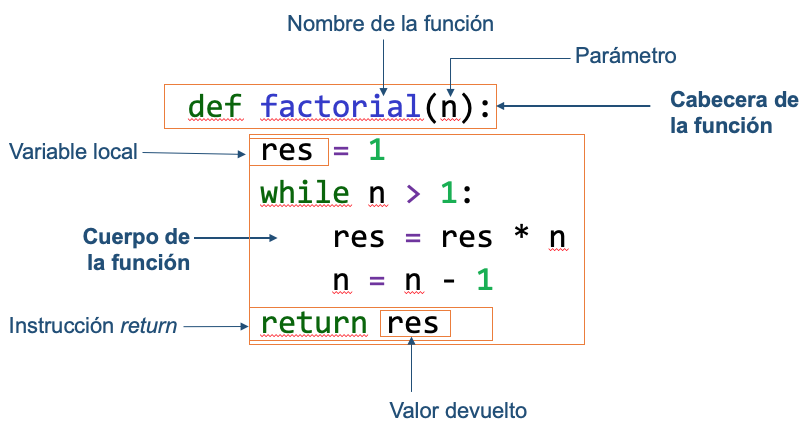
\includegraphics[width=0.75\textwidth]{images/funciones_partes.png}
    \caption{Funciones en python}
    \label{fig:partes_funciones}
\end{figure}


\index{puntos suspensivos}
Si escribes una definición de función en modo interactivo en la consola, el intérprete
mostrará puntos suspensivos (\emph{\ldots{}}) para informarte de que la
definición no está completa:

\begin{Verbatim}[frame=single]
>>> def muestra_estribillo():
...    print('A quien le importa lo que yo haga?')
...    print('A quien le importa lo que yo diga?')
...    print('Yo soy así, y así seguiré, ¡nunca cambiaré!')
\end{Verbatim}

Para finalizar la función, debes introducir una línea vacía (esto no es
necesario en un script).

Al definir una función se crea una variable con el mismo nombre.

\begin{Verbatim}[frame=single]
>>> print(muestra_estribillo)
  <function muestra_estribillo at 0xb7e99e9c>
>>> print(type(muestra_estribillo))
  <type 'function'>
\end{Verbatim}

El valor de \pythoninline{muestra\_estribillo} es \emph{function object}
(objeto función), que tiene como tipo ``function''.

\index{función, objeto} \index{objeto!función}

La sintaxis para llamar a nuestra nueva función es la misma que usamos
para las funciones predefinidas:

\begin{Verbatim}[frame=single]
>>> muestra_estribillo()
  A quien le importa lo que yo haga?
  A quien le importa lo que yo diga?
  Yo soy así, y así seguiré, nunca cambiare
\end{Verbatim}

Una vez que se ha definido una función, puede usarse dentro de otra. Por
ejemplo, para repetir el estribillo anterior, podríamos escribir una
función llamada \pythoninline{repite\_estribillo}:

\begin{python}[frame=single]
def repite_estribillo():
    muestra_estribillo()
    muestra_estribillo()
\end{python}

Y después llamar a \pythoninline{repite\_estribillo}:

\begin{Verbatim}[frame=single]
>>> repite_estribillo()
  A quien le importa lo que yo haga?
  A quien le importa lo que yo diga?
  Yo soy así, y así seguiré, ¡nunca cambiaré!
  A quien le importa lo que yo haga?
  A quien le importa lo que yo diga?
  Yo soy así, y así seguiré, ¡nunca cambiaré!
\end{Verbatim}


Reuniendo los fragmentos de código anteriores, el
programa completo sería algo como esto:

\begin{python}[frame=single]
def muestra_estribillo():
    print('A quien le importa lo que yo haga?')
    print('A quien le importa lo que yo diga?')
    print('Yo soy así, y así seguiré, ¡nunca cambiaré!')

def repite_estribillo():
    muestra_estribillo()
    muestra_estribillo()

repite_estribillo()
\end{python}

Este programa contiene dos definiciones de funciones:
\pythoninline{muestra\_estribillo} y \pythoninline{repite\_estribillo}. Las
definiciones de funciones son ejecutadas exactamente igual que cualquier
otra sentencia, pero su resultado consiste en crear objetos del tipo
función. Las sentencias dentro de cada función son ejecutadas solamente
cuando se llama a esa función, y la definición de una función no genera
ninguna salida.

\index{use before def}

Como ya te imaginarás, es necesario crear una función antes de que se
pueda ejecutar. En otras palabras, la definición de la función debe ser
ejecutada antes de que la función se llame por primera vez.

Desplazar la última línea del programa anterior
hacia arriba, de modo que la llamada a la función aparezca antes que las
definiciones. Ejecuta el programa y observa qué mensaje de error
obtienes.

Desplaza la llamada de la función de nuevo hacia el
final, y coloca la definición de \pythoninline{muestra\_estribillo} después de
la definición de \pythoninline{repite\_estribillo}. ¿Qué ocurre cuando pruebas
ese programa?

\hypertarget{flujo-de-ejecuciuxf3n}{%
\section{Flujo de ejecución}\label{flujo-de-ejecuciuxf3n}}

\index{flujo de ejecución}

Para asegurarnos de que una función está definida antes de usarla por
primera vez, es necesario saber el orden en que las sentencias son
ejecutadas, que es lo que llamamos el \emph{flujo de ejecución}.

La ejecución siempre comienza en la primera sentencia del programa. Las
sentencias son ejecutadas una por una, en orden de arriba hacia abajo.

Las \emph{definiciones} de funciones no alteran el flujo de la ejecución
del programa, pero recuerda que las sentencias dentro de una función no
son ejecutadas hasta que se llama a esa función.

Una llamada a una función es como un desvío en el flujo de la ejecución.
En vez de pasar a la siguiente sentencia, el flujo salta al cuerpo de la
función, ejecuta todas las sentencias que hay allí, y después vuelve al
punto donde lo dejó.

Todo esto parece bastante sencillo, hasta que uno recuerda que una
función puede llamar a otra. Cuando está en mitad de una función, el
programa puede tener que ejecutar las sentencias de otra función. Pero
cuando está ejecutando esa nueva función, ¡tal vez haya que ejecutar
todavía más funciones!

Afortunadamente, Python es capaz de llevar el seguimiento de dónde se
encuentra en cada momento, de modo que cada vez que completa la
ejecución de una función, el programa vuelve al punto donde lo dejó en
la función que había llamado a esa. Cuando esto le lleva hasta el final
del programa, simplemente termina.

¿Cuál es la moraleja de esta extraña historia? Cuando leas un programa,
no siempre te convendrá hacerlo de arriba a abajo. A veces tiene más
sentido seguir el flujo de la ejecución.

\hypertarget{paruxe1metros-y-argumentos}{%
\section{Parámetros y argumentos}\label{paruxe1metros-y-argumentos}}

\index{parámetro} \index{parámetro!de función} \index{argumento}
\index{argumento de función}

Algunas de las funciones predefinidas que hemos visto necesitan argumentos.
Por ejemplo, cuando se llama a \pythoninline{math.sin}, se le pasa un número
como argumento. Algunas funciones necesitan más de un argumento:
\pythoninline{math.pow} toma dos, la base y el exponente.

Dentro de las funciones, los argumentos son asignados a variables
llamadas \emph{parámetros}. A continuación mostramos un ejemplo de una
función definida por el usuario que recibe un argumento:

\index{paréntesis!parámetros entre}

\begin{python}[frame=single]
def muestra_dos_veces(bruce):
    print(bruce)
    print(bruce)
\end{python}

Esta función asigna el argumento a un parámetro llamado \pythoninline{bruce}.
Cuando la función es llamada, imprime el valor del parámetro (sea éste
lo que sea) dos veces.

Esta función funciona con cualquier valor que pueda ser mostrado en
pantalla.

\begin{Verbatim}[frame=single]
>>> muestra_dos_veces('Spam')
  Spam
  Spam
>>> muestra_dos_veces(18)
  18
  18
>>> muestra_dos_veces(math.pi)
  3.14159265359
  3.14159265359
\end{Verbatim}

Las mismas reglas de composición que se aplican a las funciones
predefinidas, también se aplican a las funciones definidas por el usuario,
de modo que podemos usar cualquier tipo de expresión como argumento para
\pythoninline{muestra\_dos\_veces}:

\index{composición}

\begin{Verbatim}[frame=single]
>>> muestra_dos_veces('Spam '*4)
  Spam Spam Spam Spam
  Spam Spam Spam Spam
>>> muestra_dos_veces(math.cos(math.pi))
  -1.0
  -1.0
\end{Verbatim}

El argumento es evaluado antes de que la función sea llamada, así que en
los ejemplos, la expresión \texttt{Spam\ *4} y
\pythoninline{math.cos(math.pi)} son evaluadas sólo una vez.

\index{argumento}

También se puede usar una variable como argumento:

\begin{Verbatim}[frame=single]
>>> michael = 'Eric, la medio-abeja.'
>>> muestra_dos_veces(michael)
  Eric, la medio-abeja.
  Eric, la medio-abeja.
\end{Verbatim}

El nombre de la variable que pasamos como argumento, (\texttt{michael})
no tiene nada que ver con el nombre del parámetro (\texttt{bruce}). No
importa cómo se haya llamado al valor en origen (en la llamada); dentro
de \texttt{muestra\_dos\_veces}, siempre se llamará \texttt{bruce}.

\hypertarget{funciones-productivas-y-funciones-estuxe9riles}{%
\section{Funciones productivas y funciones
estériles}\label{funciones-productivas-y-funciones-estuxe9riles}}

\index{productiva, función} \index{estéril, función}
\index{función productiva} \index{función esteril}

Algunas de las funciones que estamos usando, como las matemáticas,
producen resultados; a falta de un nombre mejor, las llamaremos
\emph{funciones productivas} (fruitful functions). Otras funciones, como
\pythoninline{muestra\_dos\_veces}, realizan una acción, pero no devuelven un
valor. A esas las llamaremos \emph{funciones estériles} (void
functions).

Cuando llamas a una función productiva, casi siempre querrás hacer luego
algo con el resultado; por ejemplo, puede que quieras asignarlo a una
variable o usarlo como parte de una expresión:

\begin{python}[frame=single]
x = math.cos(radians)
aurea = (math.sqrt(5) + 1) / 2
\end{python}

Cuando llamas a una función en modo interactivo, Python muestra el
resultado:

\begin{Verbatim}[frame=single]
>>> math.sqrt(5)
  2.23606797749979
\end{Verbatim}

Pero en un script, si llamas a una función productiva y no almacenas el
resultado de la misma en una variable, ¡el valor de retorno se desvanece
en la niebla!

\begin{python}[frame=single]
math.sqrt(5)
\end{python}

Este script calcula la raíz cuadrada de 5, pero dado que no almacena el
resultado en una variable ni lo muestra, no resulta en realidad muy
útil.

\index{interactivo, modo} \index{script, modo}

Las funciones estériles pueden mostrar algo en la pantalla o tener
cualquier otro efecto, pero no devuelven un valor. Si intentas asignar
el resultado a una variable, obtendrás un valor especial llamado
\pythoninline{None} (nada).

\index{None, valor especial} \index{valor especial!None}

\begin{Verbatim}[frame=single]
>>> resultado = muestra_dos_veces('Bing')
  Bing
  Bing
>>> print(resultado)
None
\end{Verbatim}

Recuerda, el valor \pythoninline{None} no es el mismo que la cadena ``None''. Es un valor especial que tiene su propio tipo:

\begin{Verbatim}[frame=single]
>>> print(type(None))
  <class 'NoneType'>
\end{Verbatim}

Para devolver un resultado desde una función, usamos la sentencia
\pythoninline{return} dentro de ella. Por ejemplo, podemos crear una función
muy simple llamada \pythoninline{sumados}, que suma dos números y devuelve el
resultado.

\begin{python}[frame=single]
def sumados(a, b):
    suma = a + b
    return suma

x = sumados(3, 5)
print(x)
\end{python}

Cuando se ejecuta este script, la sentencia \texttt{print} mostrará
``8'', ya que la función \pythoninline{sumados} ha sido llamada con 3 y 5 como
argumentos. Dentro de la función, los parámetros \pythoninline{a} y \pythoninline{b}
equivaldrán a 3 y a 5 respectivamente. La función calculó la suma de
ambos número y la guardó en una variable local a la función llamada
\pythoninline{suma}. Después usó la sentencia \pythoninline{return} para enviar el
valor calculado de vuelta al código de llamada como resultado de la
función, que fue asignado a la variable \pythoninline{x} y mostrado en
pantalla.

\hypertarget{por-quuxe9-funciones}{%
\section{¿Por qué funciones? programación modular}\label{por-quuxe9-funciones}}


La programación modular es un enfoque de diseño que divide un programa en partes pequeñas y autónomas, conocidas como módulos, cada uno de los cuales se encarga de una parte específica de la funcionalidad total del software. En este contexto, las funciones en Python se convierten en las piezas fundamentales de estos módulos, encapsulando bloques de código para realizar tareas específicas.

Cada función, como un módulo, puede ser desarrollada, probada y depurada independientemente, lo que mejora la eficiencia y \textit{reduce el riesgo de errores}. Además, una vez que una función ha sido creada y probada con éxito, se puede \textit{reutilizar} a lo largo del programa, evitando la repetición de código y asegurando la coherencia en la funcionalidad.

Este enfoque resulta en una mejora significativa de la calidad del software. Las funciones bien definidas y modulares \textit{facilitan la lectura y comprensión del código}, un factor clave en el mantenimiento y actualización de los programas. Además, la capacidad de probar y depurar funciones de manera independiente reduce la complejidad y aumenta la confiabilidad del software. En resumen, la programación modular, mediante el uso de funciones, resulta en código más limpio, eficiente, mantenible y fiable.

Una parte esencial de la programación modular, y por lo tanto del uso efectivo de las funciones, es seguir el \textit{principio de responsabilidad única}. Este principio dicta que:

\begin{center}
\fbox{\textbf{cada función debe estar encargada de una sola tarea o funcionalidad.}}
\end{center}

De esta manera, cada función se convierte en una unidad coherente y auto-contenida de código que es fácil de entender, probar y depurar.

Seguir este principio no solo mejora la legibilidad del código, sino que también aumenta su reusabilidad. Si una función se limita a realizar una única tarea, es más probable que esa función sea útil en diferentes contextos dentro del programa, y posiblemente en otros programas. Además, si una función se mantiene centrada en una sola tarea, cualquier cambio en los requisitos de esa tarea afectará solo a esa función, lo que reduce el riesgo de errores inesperados en otras partes del programa.

En resumen, el diseño de funciones que siguen el principio de responsabilidad única es un componente esencial para implementar con éxito la programación modular. Esto lleva a un código más limpio, más eficiente y más mantenible, y finalmente a un software de mayor calidad.


\begin{figure}[t]
    \centering
    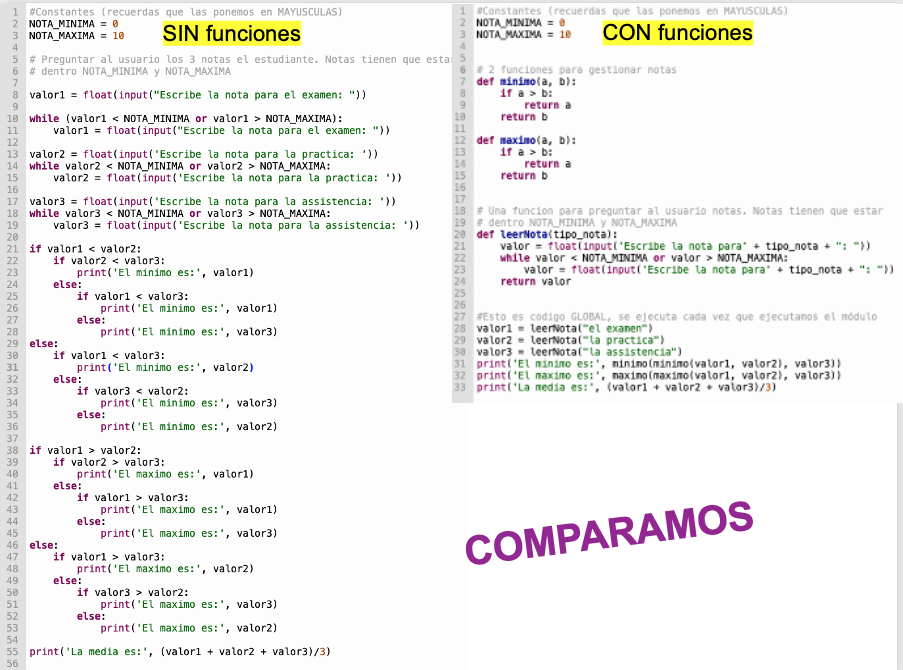
\includegraphics[width=0.85\textwidth]{images/sin-con-funciones.png}
    \caption{Comparar programa sin y con funciones.}
    \label{fig:sin.con.funciones}
\end{figure}


Algunas de estas razones lo podemos ver directamente por ejemplo en la Figura \ref{fig:sin.con.funciones} donde se puede compara 2 programas equivalentes: uno que usa funciones y la otra no.


\section{Funciones anónimas, lambda}
\index{funciones!anónimas} \index{lambda}

Las funciones lambda son funciones pequeñas y anónimas.
Las funciones lambda pueden definirse de manera rápida y concisa. Se caracterizan por no tener un nombre definido como las funciones tradicionales y se utilizan principalmente en situaciones donde se necesita una función temporal o simple que se pueda definir en el lugar donde se va a utilizar. Las Las funciones lambda son útiles especialmente cuando se necesita pasar una función como argumento a otra función.

La sintaxis básica de una función lambda es:

\begin{python}
lambda argumentos: expresión
\end{python}

donde argumentos son los parámetros que la función toma y expresión es la operación que realiza la función y devuelve su resultado. 

Por ejemplo, considera la siguiente expresión en Python:

\begin{python}
(lambda x: x ** 2)
\end{python}

esta expresión define una función lambda que calcula el cuadrado de su único argumento \pythoninline{x}. Aquí está desglosada la estructura y el significado de cada parte:

\fbox{\pythoninline{lambda}} - es la palabra clave en Python que indica que se está definiendo una función lambda, es decir, una función anónima.

\fbox{\pythoninline{x}} - es el argumento de la función lambda. En este caso, la función lambda toma un solo argumento \pythoninline{x}.

\fbox{\pythoninline{:}} (dos puntos) - marca el final de la lista de argumentos y el inicio de la expresión que define el cuerpo de la función lambda.

\fbox{\pythoninline{x ** 2}} - es la expresión que define lo que la función lambda hace con su argumento \pythoninline{x}. En este caso, eleva \pythoninline{x} al cuadrado usando el 
operador \pythoninline{**}.

Entonces, \pythoninline{(lambda x: x ** 2)} define una función anónima que toma un número como argumento \pythoninline{(x)} y devuelve su cuadrado. Esta función es anónima porque no tiene un nombre específico como las funciones definidas con def. 

La ejecución de esta expresión es por ejemplo así:

\begin{python}
>>> (lambda x: x ** 2)(4)
16

>>> (lambda x: x ** 2)(5)
25
\end{python}

Abajo hay unos ejemplos más.

\begin{python}
>>> (lambda x: x % 2 == 0)(7)
False

>>> (lambda x: x % 2 == 0)(8)
True

>>> (lambda a, b: a + " " + b) ("h", "ola")
'h ola'
\end{python}

De vez en cuando, los argumentos no se utilizan dentro de la expresión de una función lambda. En estos casos, es común utilizar un guión bajo \pythoninline{_} como nombre de variable para indicar que el valor del argumento es irrelevante para el cálculo que realiza la función lambda. Esto sirve para mantener la sintaxis de la función lambda correcta y comunicar claramente que el argumento no tiene impacto en el resultado final. Usar \pythoninline{_} de esta manera es una convención en Python que ayuda a los desarrolladores a entender rápidamente que el valor del argumento no se usa en el cuerpo de la función lambda, facilitando así el mantenimiento y la comprensión del código.

Por ejemplo:

\begin{python}
>>> (lambda _: 5)(7)
5

>>> (lambda _: 5)(100)
5
\end{python}


A continuación miramos un ejemplo que nos va a venir bien luego. Imagina que tenemos una lista con elementos:

\begin{python}
>>> ls = ['a', 'b', 'c']
\end{python}

Recuerda que el método \pythoninline{pop()} de las listas en Python es utilizado para eliminar y devolver el último elemento de la lista, o un elemento específico indicado por su índice si se proporciona. Es una operación que afecta directamente a la lista original al modificar su longitud y contenido. Cuando usas \pythoninline{pop()} sin argumentos como \pythoninline{lista.pop()}, elimina y devuelve el último elemento de la lista. Por ejemplo, llamar \pythoninline{ls.pop()} eliminará la \pythoninline{'a'} de la lista y devolverá \pythoninline{'a'}. Llamar a \pythoninline{pop()} en una lista vacía provocará un IndexError porque no hay elementos para eliminar.

Podemos definir una expresión lambda \pythoninline{(lambda _: ls.pop(0))} que cada vez que lo llamamos nos devuelve un elemento de la lista \pythoninline{ls}.

\begin{python}
>>> (lambda _: ls.pop(0))(None)
'a'
>>> (lambda _: ls.pop(0))(_)
'b'
>>> (lambda _: ls.pop(0))(8)
'c'
>>> (lambda _: ls.pop(0))("hi")
Traceback (most recent call last):
  File "<stdin>", line 1, in <module>
  File "<stdin>", line 1, in <lambda>
IndexError: pop from empty list
>>> 
\end{python}


\section{Testing nuestras funciones (el modulo pytest)}
\index{testing} \index{pytest}
Ya sabemos que todos los programas que escribimos deben ser testeados para chequear que los resultados de nuestros programas coinciden con las que esperamos. 
%
Cuando escribimos programas con los que podemos interactuar a través de la consola, podemos testear nuestro programa ingresando datos de entrada de prueba a través del teclado y verificando la salida resultante en la pantalla.
%
Sin embargo, ahora cuando escribimos funciones, podemos usar el módulo \pythoninline{pytest} para comprobar su funcionamiento.

Por ejemplo, imagina que tenemos que escribir una función \pythoninline{sin_vocales} que dado un string \pythoninline{s}, devuelve el mismo string \pythoninline{s} pero sin vocales. Por ejemplo:\\

\begin{Verbatim}[frame=single, label = {\em ejemplo de ejecución}]
>>> sin_vocales("el agua esta mojada")
  l g st mjd
\end{Verbatim}

¿Qué tests ejecutarías para probar bien tu programa? Podemos probar con:

\begin{itemize}[nosep]
    \item el string del ejemplo \texttt{''el agua esta mojada''}, 
    \item el ejemplo empieza con un vocal,vamos a hacer otro test que empieza con un consonante
    \item el ejemplo termina con un vocal,vamos a hacer otro test que termina con un consonante
    \item el string vacio,
     \item un string sin espacios,
    \item un string con solo una letra vocal,
     \item un string con solo una letra consonante,
    \item un string con mayúsculas
    \item un string que no tiene vocales
    \item un string que solo tiene vocales
    \item un string con dígitos
    \item un string con signos como interrogación
\end{itemize}

Diseñamos nuestro conjunto de tests eligiendo valores de entradas y salidas esperadas:

\begin{tabular}{|l|l|l|l|}
\hline
caso de test & entrada & salida esperada & comentario  \\ \hline\hline
1 & \verb@"el agua esta mojada"@ & \verb@"l g st mjd"@ & ejemplo del enunciado\\
2 & \verb@"mojada bañando en el agua"@ & \verb@"mjd bñnd n l g"@ & empieza con un consonante\\
3 & \verb@"ahora termina bien"@ & \verb@"hr trmn bn"@ & termina con un consonante\\
4 & \verb@""@ & \verb@""@ & el string vacio\\
5 & \verb@"a"@ & \verb@""@ & solo una letra vocal\\
6 & \verb@"m"@ & \verb@"m"@ & solo una letra consonante\\
7 & \verb@"unstringsinespacios"@ &  \verb@"nstrngsnspcs"@ & sin espacios\\
8 & \verb@"MAYUSculas FUNCIOnaN"@ & \verb@"MYScls FNCnN"@ & string con mayúsculas\\
9 & \verb@"krt yhgf dwpq"@ & \verb@"krt yhgf dwpq"@ & que no tiene vocales\\
10 & \verb@"aeoiuuuoiea"@ & \verb@""@ & que solo tiene vocales\\
11 & \verb@"disco de los 80"@ & \verb@"dsc d ls 80"@ & con dígitos\\
12 & \verb@"signos como ? y ! y ¡"@ & \verb@"sgns cm ? y ! y ¡"@ & con signos como interrogación\\
\hline
\end{tabular}

Imagina que implementamos nuestra función en un fichero \texttt{sin\_vocales.py}

\begin{python}
def sin_vocales (s):
    """
    devuelve el argumento s sin vocales
    """
    vocales = 'aeiouAEIOU'
    s_sinVocales = ''
    for ch in s:
        pos = vocales.find(ch)
        if pos == -1: #ch no es vocal
            s_sinVocales = s_sinVocales + ch     
    return s_sinVocales
\end{python}

Podemos ejecutar los tests cada uno en la consola, llamando a la función con las entradas y después chequear que lo que devuelve la función corresponda con la salida esperada:

\begin{python}
>>> sin_vocales("El agua esta mojada")
'l g st mjd'
>>> sin_vocales("mojada bañando en el agua")
'mjd bñnd n l g'
>>> 
\end{python}
\index{assert}\index{assertions}
Eso es bastante trabajo! Además, cada vez que tenemos que testear la función tenemos que repetirlo. Mejor que lo automatizamos estas llamadas con Python! 
Para eso vamos a usar \pythoninline{assert}, una instrucción en Python que se utiliza para verificar si una determinada condición es verdadera (True). Es comúnmente utilizada para realizar afirmaciones (assertions) en pruebas para verificar si un resultado esperado coincide con el resultado real.

En el contexto de pytest, una herramienta popular para realizar pruebas en Python, \pythoninline{assert} se utiliza para realizar afirmaciones dentro de las funciones de prueba. Cuando se ejecuta una prueba y se encuentra una afirmación utilizando \pythoninline{assert}, Pytest evaluará la condición y determinará si es verdadera o falsa.

Si la afirmación es verdadera, la prueba se considera exitosa y continúa ejecutándose. Sin embargo, si la afirmación es falsa, se considera un error de aserción (assertion error) y la prueba se detiene en ese punto. Pytest registra el error de aserción y proporciona información detallada sobre la prueba fallida, incluyendo la ubicación en el código y el mensaje de error asociado.

Por ejemplo los casos de test de la tabla podemos automatizar así:

\begin{python}
import pytest
def test_sin_vocales():
    assert sin_vocales("El agua esta mojada") == "l g st mjd"
    assert sin_vocales("mojada bañando en el agua") == "mjd bñnd n l g"
    assert sin_vocales("ahora termina bien") == "hr trmn bn"
    assert sin_vocales("") == ""
    assert sin_vocales("a") == ""
    assert sin_vocales("m") == "m"
    assert sin_vocales("unstringsinespacios") == "nstrngsnspcs"
    assert sin_vocales("MAYUSculas FUNCIOnaN") == "MYScls FNCnN"
    assert sin_vocales("krt yhgf dwpq") == "krt yhgf dwpq"
    assert sin_vocales("aeoiuuuoiea") == ""
    assert sin_vocales("disco de los 80") == "dsc d ls 80"
    assert sin_vocales("signos como ? y ! y ¡") == "sgns cm ? y ! y ¡"
\end{python}

Para ejecutar los tests hacemos en la consola del Thonny:

\begin{Verbatim}[frame=single]
>>> !py.test sin_vocales.py
============================= test session starts ==============================
platform darwin -- Python 3.7.9, pytest-6.1.2, py-1.9.0, pluggy-0.13.1
plugins: cov-4.0.0
collected 1 item

sin_vocales.py .                                                         [100%]

============================== 1 passed in 0.01s ===============================
>>> 
\end{Verbatim}

Podemos ver que pytest considera \pythoninline{test_sin_vocales} con sus 12 casos de test (hay 12 asserts) como 1 pytest. Vemos \pythoninline{collected 1 item} y \pythoninline{1 passed in 0.01s}.

Podemos ver que los 12 casos de test que hemos definidos han pasado. Nuestro programa ha sobrevivido los 12 tests! Ahora pensaras quizás ''pero en castellano también tenemos acentos, á, é, etc., ta,bien son vocales''. Vamos a añadir tests para estos casos:

\begin{tabular}{|l|l|l|l|}
\hline
caso de test & entrada & salida esperada & comentario  \\ \hline\hline
13 & \verb@"ábc élla óm"@ & \verb@"bc ll m"@ & acentos en minúsculas\\
14 & \verb@"Ó tambien mayÚsculÁs"@ &  \verb@"tmbn myscls"@ & acentos en mayúsculas\\
\hline
\end{tabular}


Los pytests se quedará como:


\begin{python}
def test_sin_vocales():
    assert sin_vocales("El agua esta mojada") == "l g st mjd"
    assert sin_vocales("mojada bañando en el agua") == "mjd bñnd n l g"
    assert sin_vocales("ahora termina bien") == "hr trmn bn"
    assert sin_vocales("") == ""
    assert sin_vocales("a") == ""
    assert sin_vocales("m") == "m"
    assert sin_vocales("unstringsinespacios") == "nstrngsnspcs"
    assert sin_vocales("MAYUSculas FUNCIOnaN") == "MYScls FNCnN"
    assert sin_vocales("krt yhgf dwpq") == "krt yhgf dwpq"
    assert sin_vocales("aeoiuuuoiea") == ""
    assert sin_vocales("disco de los 80") == "dsc d ls 80"
    assert sin_vocales("signos como ? y ! y ¡") == "sgns cm ? y ! y ¡"
    assert sin_vocales("ábc élla óm") == "bc ll m"
    assert sin_vocales("Óm tambien mayÚsculÁs") == "m tmbn myscls"
\end{python}

Ejecutarmos los tests en la consola del Thonny y nos sale:

\begin{footnotesize}
\begin{Verbatim}[frame=single]
>>> %Run sin_vocales.py
>>> !py.test sin_vocales.py
============================= test session starts ==============================
platform darwin -- Python 3.7.9, pytest-6.1.2, py-1.9.0, pluggy-0.13.1
plugins: cov-4.0.0
collected 1 item

sin_vocales.py F                                                         [100%]

=================================== FAILURES ===================================
_______________________________ test_sin_vocales _______________________________

    def test_sin_vocales():
        assert sin_vocales("El agua esta mojada") == "l g st mjd"
        assert sin_vocales("mojada bañando en el agua") == "mjd bñnd n l g"
        assert sin_vocales("ahora termina bien") == "hr trmn bn"
        assert sin_vocales("") == ""
        assert sin_vocales("a") == ""
        assert sin_vocales("m") == "m"
        assert sin_vocales("unstringsinespacios") == "nstrngsnspcs"
        assert sin_vocales("MAYUSculas FUNCIOnaN") == "MYScls FNCnN"
        assert sin_vocales("krt yhgf dwpq") == "krt yhgf dwpq"
        assert sin_vocales("aeoiuuuoiea") == ""
        assert sin_vocales("disco de los 80") == "dsc d ls 80"
        assert sin_vocales("signos como ? y ! y ¡") == "sgns cm ? y ! y ¡"
>       assert sin_vocales("ábc élla óm") == "bc ll m"
E       AssertionError: assert 'ábc éll óm' == 'bc ll m'
E         - bc ll m
E         + ábc éll óm

sin_vocales.py:29: AssertionError
=========================== short test summary info ============================
FAILED sin_vocales.py::test_sin_vocales - AssertionError: assert 'ábc éll óm' ...
============================== 1 failed in 0.04s ===============================
>>> 
\end{Verbatim}
\end{footnotesize}


El test ha fallado, nuestra función \pythoninline{sin_vocales} no funciona bien para los acentos en castellano. Vemos que los tests se han ejecutado hasta  \pythoninline{assert sin_vocales("ábc élla ó") == "bc ll"} es donde ha aparecido el primer error. Ya no se ha ejecutado más \pythoninline{asserts.}

Arreglamos nuestra función y añadiremos los minúsculas con acentos:


%    vocales = 'aeiouAEIOUáéóíúàèìòù'
\begin{python}
def sin_vocales (s):
    """
    devuelve el argumento s sin vocales
    """

    s_sinVocales = ''
    for ch in s:
        pos = vocales.find(ch)
        if pos == -1: #ch no es vocal
            s_sinVocales = s_sinVocales + ch     
    return s_sinVocales
\end{python}


Corremos otra ves los tests:

\begin{footnotesize}
\begin{Verbatim}[frame=single]
>>> !py.test sin_vocales.py
============================= test session starts ==============================
platform darwin -- Python 3.7.9, pytest-6.1.2, py-1.9.0, pluggy-0.13.1
plugins: cov-4.0.0
collected 1 item

sin_vocales.py F                                                         [100%]

=================================== FAILURES ===================================
_______________________________ test_sin_vocales _______________________________

    def test_sin_vocales():
        assert sin_vocales("El agua esta mojada") == "l g st mjd"
        assert sin_vocales("mojada bañando en el agua") == "mjd bñnd n l g"
        assert sin_vocales("ahora termina bien") == "hr trmn bn"
        assert sin_vocales("") == ""
        assert sin_vocales("a") == ""
        assert sin_vocales("m") == "m"
        assert sin_vocales("unstringsinespacios") == "nstrngsnspcs"
        assert sin_vocales("MAYUSculas FUNCIOnaN") == "MYScls FNCnN"
        assert sin_vocales("krt yhgf dwpq") == "krt yhgf dwpq"
        assert sin_vocales("aeoiuuuoiea") == ""
        assert sin_vocales("disco de los 80") == "dsc d ls 80"
        assert sin_vocales("signos como ? y ! y ¡") == "sgns cm ? y ! y ¡"
        assert sin_vocales("ábc élla óm") == "bc ll m"
>       assert sin_vocales("Óm tambien mayÚsculÁs") == "m tmbn myscls"
E       AssertionError: assert 'Óm tmbn myÚsclÁs' == 'm tmbn myscls'
E         - m tmbn myscls
E         + Óm tmbn myÚsclÁs
E         ? +         +   +

sin_vocales.py:30: AssertionError
=========================== short test summary info ============================
FAILED sin_vocales.py::test_sin_vocales - AssertionError: assert 'Óm tmbn myÚ...
============================== 1 failed in 0.05s ===============================
\end{Verbatim}
\end{footnotesize}

\index{AssertionError}
Ahora vemos que nos da un \pythoninline{AssertionError} para el ultimo test. Evidentemente también tenemos que añadir los mayusculas! Adaptamos nuestra función:

%'aeiouAEIOUáéóíúàèìòùÁÉÍÓÚÀÈÌÒÙ'

\begin{python}
def sin_vocales (s):
    """
    devuelve el argumento s sin vocales
    """
    vocales = 
    s_sinVocales = ''
    for ch in s:
        pos = vocales.find(ch)
        if pos == -1: #ch no es vocal
            s_sinVocales = s_sinVocales + ch     
    return s_sinVocales

\end{python}

Ejecutamos los tests:


\begin{footnotesize}
\begin{Verbatim}[frame=single]
>>> !py.test sin_vocales.py
============================= test session starts ==============================
platform darwin -- Python 3.7.9, pytest-6.1.2, py-1.9.0, pluggy-0.13.1
plugins: cov-4.0.0
collected 1 item

sin_vocales.py .                                                         [100%]

============================== 1 passed in 0.01s ===============================
>>> 
\end{Verbatim}
\end{footnotesize}

Ahora si! Los 14 tests que hemos preparado han pasado. ¿Pero son suficientes estos tests? ¿Qué mas cosas tenemos que probar?

\index{diéresis}
La diéresis es, según la Real Academia Española (RAE), “un signo ortográfico auxiliar representado por dos puntos (¨) que se disponen horizontalmente sobre la vocal a la que afectan”. Este signo también se llama crema, y en español se escribe siempre sobre una vocal de la siguiente manera: ä, ë, ï, ö, ü. Estos también tenemos que añadir. ¿Que casos de test se nos ocurre más?

En la sección \ref{test-mnemonic} vemos una mnemónica para ayudarnos a pensar mejor en que casos de test diseñar.


\section{Testing de funciones que lanzan excepciones}\label{test-excep}

Consideramos la siguiente función \pythoninline{check_input} que lanza excepciones:

\begin{python}
def check_input(n):
    if not (type(n) == int or type(n) == float):
        raise ValueError("Wrong Type")
    elif (int(n) != n) or (n <= 0):
        raise ValueError("Wrong Value")
\end{python}

Cuando esta función recibe un argumento que tiene el \textbf{tipo} que no es numerico (bool, strings, etc) devolverá una excepción \pythoninline{ValueError("Wrong Type")}. Cuando recibe un 0 o números negativos o floats con parte decimal no igual a 0  devolverá una excepción \pythoninline{ValueError("Wrong Value")}. Cuando el valor es correcto, no devuelve nada (es decir \pythoninline{None}).

\index{pytest.raises}
Para testear una función que puede lanzar excepciones podemos usar \pythoninline{pytest.raises}, este concepto de pytest nos permite verificar si una determinada excepción se lanza en un código. Es útil para escribir pruebas cuando esperamos que una función genere una excepción en ciertas situaciones. Por ejemplo, para testear que \pythoninline{check_input} lanza un \pythoninline{ValueError} cuando su argumento es 0, podemos definir:

\begin{python}
def test_check_input():
    with pytest.raises(ValueError):
        assert check_input(0)
\end{python}

Si también queremos testear el mensaje de la excepción, podemos capturar la excepción utilizando una variable dentro del contexto. Luego, podemos acceder a los atributos de esa excepción para obtener información específica. Por ejemplo:

\begin{python}
def test_check_input():
   with pytest.raises(ValueError) as excinfo:
        assert check_input(0)
   assert str(excinfo.value) == "Wrong Value"
\end{python}

La implementacion de los siguientes tests:

\begin{longtable}{|l|l|l|}
\hline
testcase número & argumento & output esperado  \\ \hline
1  &  0       & \pythoninline{ValueError("Wrong Value")} \\ 
2  & 97.2     & \pythoninline{ValueError("Wrong Value")} \\
3  &  \pythoninline{'a'}    & \pythoninline{ValueError("Wrong Type")}\\
4  &  -3     &  \pythoninline{ValueError("Wrong Value")} \\
5  & \pythoninline{True}  &  \pythoninline{ValueError("Wrong Type")}\\
6  & 1 & \pythoninline{None}\\
7  & 25 & \pythoninline{None}\\
10  & 25.0 & \pythoninline{None}\\
11  & 25.000 & \pythoninline{None}\\
\hline
\end{longtable}

esta abajo:\\

\begin{python}
def test_check_input():

    with pytest.raises(ValueError):
        assert check_input_for_es_primo(0)

    #Si también queremos testear el mensaje de la excepción
    with pytest.raises(ValueError) as excinfo:
        assert check_input_for_es_primo(0)
    assert str(excinfo.value) == "Wrong Value"
    
    with pytest.raises(ValueError):
        assert check_input_for_es_primo(97.2)

    with pytest.raises(ValueError):
        assert check_input_for_es_primo("a")

    with pytest.raises(ValueError):
        assert check_input_for_es_primo("-3")

    with pytest.raises(ValueError):
        assert check_input_for_es_primo(True)
    
    #Si también queremos testear el mensaje de la excepción
    with pytest.raises(ValueError) as excinfo:
         assert check_input_for_es_primo(True)
    assert str(excinfo.value) == "Wrong Type"
    
    assert check_input_for_es_primo(1)    == None
    assert check_input_for_es_primo(2)    == None
    assert check_input_for_es_primo(25)   == None
    assert check_input_for_es_primo(25.0)   == None
    assert check_input_for_es_primo(25.000)   == None
\end{python}

%%%%


\index{CODE mnemónica}\index{mnemónica CODE}
\section{CODE, una mnemónica para testing}\label{test-mnemonic}
\index{mnemonic}

Para tener un poco más de guía para saber qué casos de tests probar con tu programa, podemos usar el mnemónica CODE:

\begin{description}
\item[{\color{red} C}]ardinalidad
\item[{\color{red} O}]rden
\item[{\color{red} D}]ominio
\item[{\color{red} E}]structura
\end{description}

Este mnemónica esta inspirado por el libro de Jeff Langr, {\em Pragmatic Unit testing un Java with Junit.}. Las palabras que componen la mnemónica nos puede servir de ayuda para generar ideas en cuanto a que entradas probar, solo eso. No esta garantizado que nos surgen ideas, ni que se aplica a todas las posibles funciones, pero siempre es útil poder empezar con algo que te puede generar ideas.

\subsection{{\color{red} C}ardinalidad}

En matemáticas, la cardinalidad de un valor es la medida del "número de elementos". Por ejemplo, el string \pythoninline{'abcd'} contiene 4 letras, y por tanto tiene cardinalidad 4. Esta parte del mnemónica nos recuerda probar diferentes cardinalidades de las entradas. Por ejemplo,

\begin{itemize}
    \item cardinalidad 0
    \item cardinalidad 1
    \item cardinalidad > 1
\end{itemize}

Recordamos la función \pythoninline{sin_vocales} que dado un string \pythoninline{s}, devuelve el mismo string \pythoninline{s} pero sin vocales.

\begin{Verbatim}[frame=single, label = {\em ejemplo de ejecución}]
>>> sin_vocales("el agua esta mojada")
  l g st mjd
\end{Verbatim}

De los casos de test que vimos antes, los que comprueban diferentes cardinalidades para \pythoninline{s} son:

\begin{tabular}{|l|l|l|l|}
\hline
caso de test & entrada & salida esperada & comentario  \\ \hline\hline
1 & \verb@"el agua esta mojada"@ & \verb@"l g st mjd"@ & cardinalidad \pythoninline{s} > 1\\
4 & \verb@""@ & \verb@""@ & el string vacio, cardinalidad \pythoninline{s} = 0\\
5 & \verb@"a"@ & \verb@""@ & cardinalidad \pythoninline{s} = 1, letra es vocal\\
6 & \verb@"m"@ & \verb@"m"@ & cardinalidad \pythoninline{s} = 1, letra no es vocal\\
\hline
\end{tabular}


La heurística de la cardinalidad nos ayuda a considerar casos de prueba que cubren diferentes números de elementos en nuestras entradas, lo que nos permite identificar posibles problemas con nuestros programas en diferentes situaciones. 


\subsection{{\color{red} O}rden}

Para algunas funciones y sus soluciones, el orden de los elementos es importante, mientras que para otras no lo es. En ambos casos, es necesario probar que el método funciona correctamente.

Recordamos la función \pythoninline{sin_vocales} que dado un string \pythoninline{s}, devuelve el mismo string \pythoninline{s} pero sin vocales.

De los casos de test que vimos antes, que comprueban diferentes orden de donde están los vocales para \pythoninline{s} son:

\begin{tabular}{|l|l|l|l|}
\hline
caso de test & entrada & salida esperada & comentario  \\ \hline\hline
1 & \verb@"el agua esta mojada"@ & \verb@"l g st mjd"@ & empieza y termina con vocal\\
2 & \verb@"mojada bañando en el agua"@ & \verb@"mjd bñnd n l g"@ & empieza con un consonante\\
3 & \verb@"ahora termina bien"@ & \verb@"hr trmn bn"@ & termina con un consonante\\
\hline
\end{tabular}


La heurística {\color{red} O}rden nos guía para probar diferentes disposiciones o secuencias de elementos en las entradas. Al considerar diversos órdenes, podemos asegurarnos de que nuestro programa maneje correctamente las variaciones en la disposición de los datos."



\subsection{{\color{red} D}ominio}

Hay que pensar si es necesario probar con diferentes dominios de los parámetros y sus limites.

La especificación de la función \pythoninline{sin_vocales} dice claramente que tiene que funcionar cuando le damos un argumento de tipo string \pythoninline{s}. Entonces, realmente no hace falta que funciona para tipo int, float, etc. porque no es lo que promete la función. Lo que si podemos hacer es probar con strings que contienen números, para verificar que nuestra función funciona y no por ejemplo lo detecta como vocales o algo así.

De los casos de test que vimos antes, los que comprueban diferentes orden de donde están los vocales para \pythoninline{s} son:

\begin{tabular}{|l|l|l|l|}
\hline
caso de test & entrada & salida esperada & comentario  \\ \hline\hline
11 & \verb@"disco de los 80"@ & \verb@"dsc d ls 80"@ & con dígitos\\
\hline
\end{tabular}


\subsection{{\color{red} E}structura}

La estructura de los parámetros puede ser muy importante para el buen funcionamiento de una función. Vemos que para la función \pythoninline{sin_vocales} y el argumento \pythoninline{s} de tipo string, el resto de los casos de test que vimos antes, comprueban diferentes estructuras de la string \pythoninline{s} son:

\begin{tabular}{|l|l|l|l|}
\hline
caso de test & entrada & salida esperada & comentario  \\ \hline\hline
7 & \verb@"unstringsinespacios"@ &  \verb@"nstrngsnspcs"@ & sin espacios\\
8 & \verb@"MAYUSculas FUNCIOnaN"@ & \verb@"MYScls FNCnN"@ & string con mayúsculas\\
9 & \verb@"krt yhgf dwpq"@ & \verb@"krt yhgf dwpq"@ & que no tiene vocales\\
10 & \verb@"aeoiuuuoiea"@ & \verb@""@ & que solo tiene vocales\\
12 & \verb@"signos como ? y ! y ¡"@ & \verb@"sgns cm ? y ! y ¡"@ & con signos como interrogación\\
\hline
\end{tabular}

\subsection{Ejemplo para otra función}

Imagina que tenemos que escribir una función que dado una cadena de texto, devuelve la cantidad de números que aparecen en la cadena. Nota: Con número no queremos decir dígito, sino número propiamente dicho, es decir, secuencia de dígitos. La cadena `un 1, un 201 y 2 unos', por ejemplo, tiene 3 números: el 1, el 201 y el 2.

\subsubsection{{\color{red} C}ardinalidad}

Exploramos diferentes números de elementos en las entradas para verificar cómo responde nuestra función.\\

\begin{tabular}{|l|l|l|l|}
\hline
Caso de prueba & Entrada & Salida esperada & Comentario  \\ \hline\hline
1 & \verb@"un 1, un 201 y 2 unos"@ & 3 & Varios números en la cadena\\
2 & \verb@"sin numeros"@ & 0 & Sin números en la cadena\\
3 & \verb@"2345543"@ & 1 & Un solo número en la cadena\\
4 & \verb@"1 22 333 4444 55555"@ & 5 & Diferentes longitudes de números\\
\hline
\end{tabular}

\subsubsection{{\color{red} O}rden}

Consideramos el orden de los números y su posición en la cadena.\\

\begin{tabular}{|l|l|l|l|}
\hline
Caso de prueba & Entrada & Salida esperada & Comentario  \\ \hline\hline
5 & \verb@"123 456 789"@ & 3 & Números separados por espacios\\
6 & \verb@"12,34,56,78"@ & 4 & Números separados por comas\\
7 & \verb@"numero123numero456numero"@ & 2 & Números rodeados de texto\\
8 & \verb@"123456789"@ & 1 & Una cadena continua de números\\
9 & \verb@"1 starting and ending 2"@ & 2 & Números al inicio y al final\\
10 & \verb@"ending with number 5"@ & 1 & Número al final\\
\hline
\end{tabular}

\subsubsection{{\color{red} D}ominio}

Es importante probar diferentes dominios de cadenas de entrada.\\

\begin{tabular}{|l|l|l|l|}
\hline
Caso de prueba & Entrada & Salida esperada & Comentario  \\ \hline\hline
11 & \verb@"3 6 9"@ & 3 & Números en una cadena simple\\
12 & \verb@"sinnumeros"@ & 0 & Sin números en la cadena\\
13 & \verb@"123unnumero456"@ & 2 & Números mezclados con texto\\
14 & \verb@"-5 10 -15"@ & 3 & Números negativos\\
\hline
\end{tabular}

\subsubsection{{\color{red} E}structura}

La estructura de los parámetros en este caso es similar al orden en que aparecen los numeros. Por ejemplo:\\

\begin{tabular}{|l|l|l|l|}
\hline
Caso de prueba & Entrada & Salida esperada & Comentario  \\ \hline\hline
15 & \verb@"123 456 789"@ & 3 & Números separados por espacios\\
16 & \verb@"12,34,56,78"@ & 4 & Números separados por comas\\
17 & \verb@"numero123numero456numero"@ & 2 & Números rodeados de texto\\
18 & \verb@"123456789"@ & 1 & Una cadena continua de números\\
\hline
\end{tabular}

La implementación en python de la función y los pytests esta en la Figura \ref{test_cantidad_de_nums}.

\begin{figure}[T]
\begin{python}
import pytest

def cantidad_de_nums(n):
    """una función que dado una cadena de texto,
    devuelve la cantidad de ńumeros que aparecen
    en la cadena
    """
    
    lista = []
    RN = False #bandera para saber si estamos Recorriendo un Numero
    cantidad = 0

    n = n +"." #añadir algo que no es digito al final 

    for i in n:
        if i.isdigit():
            RN = True #todavia recorriendo numero
        elif RN == True:
            cantidad += 1
            RN = False #ya no recorriendo numero
            
    return cantidad

def test_cantidad_de_nums():
    # Casos para Cardinalidad
    assert cantidad_de_nums("un 1, un 201 y 2 unos") == 3
    assert cantidad_de_nums("sin numeros") == 0
    assert cantidad_de_nums("2345543") == 1
    assert cantidad_de_nums("1 22 333 4444 55555") == 5
    
    # Casos para Orden
    assert cantidad_de_nums("123 456 789") == 3
    assert cantidad_de_nums("12,34,56,78") == 4
    assert cantidad_de_nums("numero123numero456numero") == 2
    assert cantidad_de_nums("123456789") == 1
    assert cantidad_de_nums("1 starting and ending 2") == 2
    assert cantidad_de_nums("ending with number 5") == 1
    
    # Casos para Dominio
    assert cantidad_de_nums("3 6 9") == 3
    assert cantidad_de_nums("sinnumeros") == 0
    assert cantidad_de_nums("123unnumero456") == 2
    assert cantidad_de_nums("-5 10 -15") == 3
    
    # Casos para Estructura
    assert cantidad_de_nums("123 456 789") == 3
    assert cantidad_de_nums("12,34,56,78") == 4
    assert cantidad_de_nums("numero123numero456numero") == 2
    assert cantidad_de_nums("123456789") == 1
\end{python}
\caption{pytests for \textbf{cantidad\_de\_nums}}
\label{test_cantidad_de_nums}
\end{figure}


\index{pytest.mark.parametrize}
\section{Parametrizar los pytests}

También podemos usar \pythoninline{pytest.mark.parametrize} para definir los casos de tests (i.e. las entradas y salidas esperadas) que queremos ejecutar, pero como parámetros de un driver de test.
%
Este tiene algunos ventajas, pero si ya te parece difícil lo de los tests, deja esto para mas tarde.

Recuerda los pytests en \pythoninline{test_sin_vocales}:

\begin{python}
def test_sin_vocales():
    assert sin_vocales("El agua esta mojada") == "l g st mjd"
    assert sin_vocales("mojada bañando en el agua") == "mjd bñnd n l g"
    assert sin_vocales("ahora termina bien") == "hr trmn bn"
    assert sin_vocales("") == ""
    assert sin_vocales("a") == ""
    assert sin_vocales("m") == "m"
    assert sin_vocales("unstringsinespacios") == "nstrngsnspcs"
    assert sin_vocales("MAYUSculas FUNCIOnaN") == "MYScls FNCnN"
    assert sin_vocales("krt yhgf dwpq") == "krt yhgf dwpq"
    assert sin_vocales("aeoiuuuoiea") == ""
    assert sin_vocales("disco de los 80") == "dsc d ls 80"
    assert sin_vocales("signos como ? y ! y ¡") == "sgns cm ? y ! y ¡"
\end{python}

Los podemos parametrizar así:

\begin{python}
import pytest
@pytest.mark.parametrize("entrada, salida_esperada",[
("El agua esta mojada", "l g st mjd"),           
("mojada bañando en el agua", "mjd bñnd n l g"),
("ahora termina bien", "hr trmn bn"),
("", ""),                                       
("a", ""), 
("m", "m"), 
("unstringsinespacios", "nstrngsnspcs"),        
("MAYUSculas FUNCIOnaN", "MYScls FNCnN"),       
("krt yhgf dwpq", "krt yhgf dwpq"),             
("aeoiuuuoiea", ""),                            
("disco de los 80", "dsc d ls 80"),             
("signos como ? y ! y ¡", "sgns cm ? y ! y ¡")   
])

def test_sin_vocales(entrada, salida_esperada):
    assert sin_vocales(entrada) == salida_esperada
\end{python}

El primer argumento de \pythoninline{pytest.mark.parametrize}, es decir: \pythoninline{'entrada, salida_esperada'}, refleja los componentes de los casos de test para esta función. Esto se llama 
\emph{test signature} y para esta función corresponde con las columnas \textit{entrada} y \textit{salida esperada} de nuestra tabla de arriba.

\begin{itemize}
    \item \pythoninline{'entrada'}: la entrada que queremos dar a la función
    \item \pythoninline{'salida_esperada'}: la salida que esperamos que sale
\end{itemize}

El resto de los argumentos de \pythoninline{pytest.mark.parametrize} consiste de los casos de test que hemos definidos.

\index{test signature}
Después definimos una función de prueba \pythoninline{test_sin_vocales} que recibe una cantidad de parámetros que coincide con el \emph{test signature}. El unico que hace la función es:

\begin{itemize}
    \item llamar a la función que queremos testear con las entradas \pythoninline{sin_vocales(entrada)}
    \item comparar lo que sale con la salida esperada \pythoninline{== salida_esperada}
    \item cuando la instrucción \pythoninline{assert} recibe un \pythoninline{True} (que significa que lo que ha salido de la función es lo que esperábamos) no hace nada.
    \item cuando la instrucción \pythoninline{assert} recibe un \pythoninline{False} (que significa que NO ha salido lo que esperábamos) entonces lanza un error de aserción.
\end{itemize}


El modulo \pythoninline{pytest} asegura que la función de prueba recibe todos los casos de test definidos en \pythoninline{pytest.mark.parametrize}. Para ejecutar los tests hacemos en la consola del Thonny:


\begin{Verbatim}[frame=single]
>>> !py.test sin_vocales.py
============================= test session starts ==============================
platform darwin -- Python 3.7.9, pytest-6.1.2, py-1.9.0, pluggy-0.13.1
collected 12 items

sin_vocales.py ........                                                    [100%]
============================== 12 passed in 0.02s ===============================
\end{Verbatim}

Con \pythoninline{pytest.mark.parametrize} vemos que pytest considera los 12 asserts por separado. Vemos que pone \texttt{collected 12 items} y \texttt{12 passed in 0.02s}. Eso es una diferencia de las 2 formas de definir de tests.




\section{Testing de funciones estériles}

Consideramos la siguiente función \pythoninline{main} que lea un carácter desde teclado y determine con la función \pythoninline{es_digito} si se trata de uno de los dígitos del 0 al 9. 

\begin{python}
def es_digito(n):
    if (len(n) > 1):
        return False
    elif (n.isdigit()):
        return True
    else:
        return False

def main():
    n = input("Escribe un caracter o 'fin' para terminar: ")
    if (es_digito(n)):
        print(n, "es un digito de 0 a 9")
    else:
        print(n, "no es un digito de 0 a 9")
\end{python}

La función \pythoninline{es_digito} es productiva y la podemos testear así:

\begin{python}
def test_es_digito():
    assert es_digito('0') ==  True,   "test1: digito mas pequeño"
    assert es_digito('9') ==  True,   "test2: digito mas grande"
    assert es_digito('5') ==  True,   "test3: otro digito"
    assert es_digito('12') ==  False, "test4: no es un digito entre de 0 y 9"
    assert es_digito('-2') ==  False, "test5: digito negativo"
    assert es_digito('hello') ==  False, "test6: string"
\end{python}

La función \pythoninline{main()} es estéril y se encarga de la interacción con el usuario a través del la consola. Para poder testearlo de forma automática sin necesidad de un usuario que teclea el \pythoninline{input} necesitamos hacer 2 cosas:

\begin{enumerate}
\item similar el usuario que entra datos en la consola
\item recoger los resultados de la consola
\end{enumerate}

\underline{\textbf{1) para simular el usuario necesitamos saber de 2 cosas:}}

\begin{description}
\item[mocking] implica crear un objeto falso (mock)\index{mock} que imita el comportamiento de un objeto real de manera controlada. Los objetos mock pueden ser configurados para devolver valores específicos y pueden tener sus llamadas y respuestas verificadas para asegurar que se comportan como se espera en el contexto de la prueba.\index{mocking}

\item[patching] se refiere a la técnica de modificar dinámicamente una función durante el testing. Esto puede implicar reemplazar una función real con un mock o con otro comportamiento definido por el tester.\index{patching}
\end{description}

El pytest nos ofrece para hacer esto el.\textbf{monkeypatching}\index{monkeypatching}\index{\pythoninline{monkeypatch}}
El monkey patching consiste en alterar temporalmente el comportamiento de una función mientras se está ejecutando, sin modificar directamente su implementación original. Esto facilita ajustar el comportamiento y los resultados de la función parcheada durante pruebas, permitiendo simular diversas situaciones. Es crucial recordar que el monkey patching se emplea principalmente en entornos de pruebas y no se aconseja su uso extensivo en implementaciones de producción.

Por ejemplo, el siguiente código utiliza el concepto de monkey patching para modificar temporalmente el comportamiento de la función \pythoninline{input} del módulo builtins. La función que utilizamos en el \pythoninline{main()} para pedir datos al usuario a través de la consola.

\begin{python}\index{\pythoninline{monkeypatch.setattr}}
# Simular el user input. En lugar de hacer lo que hace el built-in
# input normalmente, ahora en la simulación siempre devuelve el mock 4

monkeypatch.setattr('builtins.input', lambda _: '4')
\end{python}

El método \pythoninline{monkeypatch.setattr()} de pytest se utiliza para cambiar el comportamiento de una función en tiempo de ejecución. Lo que hace específicamente es reemplazar la función \pythoninline{input} por una función lambda que siempre devuelve la cadena \pythoninline{'4'} cuando se llama. En términos prácticos, esto simula que, en cualquier parte del código donde se llame a \pythoninline{input()}, el valor devuelto será siempre \pythoninline{'4'} en lugar de esperar una entrada del usuario.

Ya que podemos similar que el usuario que entra datos en la consola, nos queda:

\underline{\textbf{2) recoger los resultados de la consola poder chequear-los con \pythoninline{assert}}}

Para recoger datos que han sido imprimido en la consola utilizamos el fixture \pythoninline{capsys}.\index{fixture}\index{\pythoninline{capsys}}

El fixture \pythoninline{capsys} es utilizado para capturar todo lo que se imprima en la salida estándar (stdout) durante la ejecución de una prueba. Cuando se usa \pythoninline{capsys} como un fixture en un entorno de test, permite a los testers capturar y verificar las salidas generadas por funciones o métodos que imprimen texto en la consola.

El fixture \pythoninline{capsys} proporciona dos atributos principales: 
 \pythoninline{capsys.readouterr()}, \index{\pythoninline{capsys.readouterr()}}
que retorna una tupla con dos cadenas que representan lo que se ha capturado en \pythoninline{stdout} y \pythoninline{stderr} respectivamente,\index{\pythoninline{stdout}}\index{\pythoninline{stderr}}
y \pythoninline{capsys.disabled()},\index{\pythoninline{capsys.disabled()}}
que restaura la salida estándar y la estándar de error a su estado original. Esto es útil para verificar o asercionar la salida esperada de una función sin alterar la forma en que el programa interactúa normalmente con la consola durante la ejecución de pruebas unitarias.

Ahora un test de \pythoninline{main()} puede quedar así:

\begin{python}
def test_main(monkeypatch, capsys): 

    # Simular el user input. En lugar de hacer lo que hace el built-in
    # input normalmente, ahora en la simulación siempre devuelve el mock 4
    monkeypatch.setattr('builtins.input', lambda _: '4')
    
    # con 4 el valor esperado es
    expected_output = "4 es un digito de 0 a 9"
    
    #call the function
    main()
    
    #get the output
    captured = capsys.readouterr()
    
    #check
    assert captured.out.strip() == expected_output
\end{python}

Veamos qué hace cada línea de este código en detalles:

\fbox{\pythoninline{def test_main(monkeypatch, capsys)}} - Esta es la definición de la función de prueba. \pythoninline{monkeypatch} y \pythoninline{capsys} son dos fixtures proporcionados por el marco de pruebas pytest en Python. 

\begin{itemize}
\item \pythoninline{monkeypatch} se usa para modificar comportamientos dinámicamente, es decir, durante la ejecución de la prueba
\item \pythoninline{capsys} se usa para capturar salidas a stdout.    
\end{itemize}

\fbox{\pythoninline{monkeypatch.setattr('builtins.input', lambda _: '4')}} - En esta línea, usamos el fixture \pythoninline{monkeypatch} para modificar el comportamiento de la función input incorporada de Python. En lugar de esperar a que el usuario ingrese un valor, simplemente queremos que siempre devuelve "4". Esto se hace para simular la entrada del usuario durante la prueba. 

Normalmente, la función input detiene la ejecución de tu programa y espera que el usuario introduzca algo. Eso no es muy útil en una prueba automatizada. Entonces, se reemplaza con una función diferente que no espera la entrada del usuario. Aquí es donde entra en juego la función lambda. \pythoninline{lambda _: '4'} es una simple función anónima que toma un argumento \pythoninline{(_)} y siempre devuelve el string \pythoninline{'4'}. El \pythoninline{_} es una convención común en Python para una variable que no nos importa y no vamos a usar.

Por lo tanto, en efecto, esta línea de código hace que, dentro de esta prueba, cada vez que se llama a la función input, en lugar de esperar la entrada del usuario, devuelve inmediatamente el string "4". De esa manera, puedes probar cómo se comporta tu código cuando el usuario introduce "4".

\fbox{\pythoninline{expected_output = '4 es un digito de 0 a 9'}} - Aquí, simplemente estamos definiendo cuál sería la salida esperada si el usuario ingresara \pythoninline{'4'}.

\fbox{\pythoninline{main()}} - Esta es la llamada a la función que estamos probando.

\fbox{\pythoninline{captured = capsys.readouterr()}} -  Aquí, estamos utilizando el fixture \pythoninline{capsys} para capturar todo lo que se haya impreso a stdout durante la ejecución de la prueba.

\fbox{\pythoninline{assert captured.out.strip() == expected_output}} - Por último, esta es la afirmación de prueba real. Estamos comprobando que la salida de la función \pythoninline{main} coincide con la salida esperada que definiste antes.

Entonces, en resumen, este código está simulando una entrada del usuario de \pythoninline{'4'} a la función \pythoninline{main}, luego verifica que la salida de la función es \pythoninline{'4 es un digito de 0 a 9}. Es una forma de comprobar automáticamente que tu función está comportándose como se espera cuando se le da una entrada específica.


Imagina que extendemos la función \pythoninline{main} de tal forma sirva para leer varios caracteres diferentes desde teclado hasta el usuario escribe la palabra fin.

\begin{python}
def main2():
    n = input("Escribe un caracter o 'fin' para terminar: ")
    while not (n=="fin"):
        if (es_digito(n)):
            print(n, "es un digito de 0 a 9")
        else:
            print(n, "no es un digito de 0 a 9")
        n = input("Escribe un caracter o 'fin' para terminar: ")
\end{python}

Una ejecución de esta programa seria como:\\

\begin{Verbatim}[frame=single, label={\em ejemplos de test}]
>>> %Run 
  Escribe un caracter o 'fin' para terminar: 4
  4 es un digito de 0 a 9
  Escribe un caracter o 'fin' para terminar: -1
  -1 no es un digito de 0 a 9
  Escribe un caracter o 'fin' para terminar: z
  z no es un digito de 0 a 9
  Escribe un caracter o 'fin' para terminar: 56
  56 no es un digito de 0 a 9
  Escribe un caracter o 'fin' para terminar: dfg
  dfg no es un digito de 0 a 9
  Escribe un caracter o 'fin' para terminar: 0
  0 es un digito de 0 a 9
  Escribe un caracter o 'fin' para terminar: fin
>>>    
\end{Verbatim}

Cuando queremos probar esta ejecución en un test automatizado sin tener que introducir esas entradas manualmente cada vez, necesitamos asegurarnos de que hemos definido la lista \pythoninline{inputs} que contiene todos los valores de entrada que tu programa necesita.

Después definimos la función anónima \pythoninline{lambda _: inputs.pop(0)} que ignora su entrada (nuevamente, el \pythoninline{_} es una convención que indica que no nos importa el valor de entrada) y en su lugar devuelve el primer elemento de la lista \pythoninline{inputs}, y luego lo elimina de la lista. \pythoninline{pop(0)} es una operación en listas en Python que elimina y devuelve el primer elemento de la lista.

Esto significa que cada vez que tu código llame a la función \pythoninline{input()}, en lugar de esperar a que el usuario escriba algo, tu programa obtendrá el siguiente elemento de la lista \pythoninline{inputs}. La primera vez que llames a \pythoninline{input()}, obtendrás \pythoninline{inputs[0]}, la segunda vez obtendrás \pythoninline{inputs[1]}, y así sucesivamente.

El código queda así:

\begin{small}
\begin{python}
def test_main2(monkeypatch, capsys): 
    
    inputs = ['4', '-1', 'z', '56', 'dfg', '0', 'fin'] 
    
    # Mock the user input. En lugar de hacer lo que hace el built-in
    # input normalmente, ahora coge (pop) cada vez un valor de la lista inputs
    monkeypatch.setattr('builtins.input', lambda _: inputs.pop(0))
    
    #call the function
    main2()
    
    #get the output
    captured = capsys.readouterr().out
    
    #check por ejemplo que aparece 4 veces la palabra "no"
    assert captured.count("no") == 4
\end{python}
\end{small}



\section{docstring}
\label{docstring}
\index{docstring}

Un \textbf{docstring} es una cadena al comienzo de una función que
explica para que se puede usar la función (``doc'' es la abreviatura de ``documentation'').  Aquí hay un ejemplo:

\begin{python}
def minimo(a, b):
    """
    Devuelve el minimo de los dos numeros dados.
    """
    if a > b:
        return a
    return b
\end{python}
%
Por convención, todos los docstrings son cadenas entre triple comillas, también conocidas
como cadenas multilínea porque las triple comillas permiten expandir
la cadena a más de una línea.
\index{comillas}
\index{cadena!entre triple comillas}
\index{triple comillas, cadena entre}
\index{cadena!multilínea}
\index{multilínea, cadena}

Es breve, pero contiene la información esencial
que alguien necesitaría para utilizar esta función.  Explica de manera concisa lo que
hace la función (sin entrar en detalles sobre cómo lo
hace).  Explica qué efecto tiene cada parámetro en el comportamiento de
la función y de qué tipo debería ser cada parámetro (si no es
obvio).

Escribir este tipo de documentación es una parte importante del diseño de la función.  Una función bien diseñada debería ser simple de explicar; si tienes dificultades al explicar una de tus funciones, quizás la interfaz podría mejorar.

Los docstrings son accesibles con la función predefinido 
\pythoninline{help}.

\begin{Verbatim}[frame=single]
>>> help(minimo)
Help on function minimo in module __main__:

minimo(a, b)
    Devuelve el minimo de los dos numeros dados.
\end{Verbatim}



\hypertarget{editor}{%
\section{Depuración}\label{editor}}

\index{depuración}

Si estás usando un editor de texto para escribir tus propios scripts,
puede que tengas problemas con los espacios y tabulaciones. El mejor
modo de evitar esos problemas es usar espacios exclusivamente (no
tabulaciones). La mayoría de los editores de texto que reconocen Python
lo hacen así por defecto, aunque hay algunos que no.

\index{espacio en blanco}

Las tabulaciones y los espacios normalmente son invisibles, lo cual hace
que sea difícil depurar los errores que se pueden producir, así que
mejor busca un editor que gestione el indentado por ti.

Tampoco te olvides de guardar tu programa antes de hacerlo funcionar.
Algunos entornos de desarrollo lo hacen automáticamente, pero otros no.
En ese caso, el programa que estás viendo en el editor de texto puede no
ser el mismo que estás ejecutando en realidad.

¡La depuración puede llevar mucho tiempo si estás haciendo funcionar el
mismo programa con errores una y otra vez!

Asegúrate de que el código que estás examinando es el mismo que estás
ejecutando. Si no estás seguro, pon algo como \texttt{print("hola")} al
principio del programa y hazlo funcionar de nuevo. Si no ves
\texttt{hola} en la pantalla, ¡es que no estás ejecutando el programa
correcto!

\hypertarget{glosario}{%
\section{Glosario}\label{glosario}}

\begin{description}
\item[algoritmo]
Un proceso general para resolver una categoría de problemas.
\end{description}

\index{algoritmo}

\begin{description}
\item[argumento]
Un valor proporcionado a una función cuando ésta es llamada. Ese valor
se asigna al parámetro correspondiente en la función.
\end{description}

\index{argumento}

\begin{description}
\item[cabecera]
La primera línea de una definición de función.
\end{description}

\index{cabecera}

\begin{description}
\item[cuerpo]
La secuencia de sentencias dentro de la definición de una función.
\end{description}

\index{cuerpo}

\begin{description}
\item[composición]
Uso de una expresión o sentencia como parte de otra más larga,
\end{description}

\index{composición}

\begin{description}
\item[definición de función]
Una sentencia que crea una función nueva, especificando su nombre,
parámetros, y las sentencias que ejecuta.
\end{description}

\index{función, definición}

\begin{description}
\item[determinístico]
Perteneciente a un programa que hace lo mismo cada vez que se ejecuta, a
partir de las mismas entradas.
\end{description}

\index{determinístico}

\begin{description}
\item[función]
Una secuencia de sentencias con un nombre que realizan alguna operación
útil. Las funciones pueden tomar argumentos o no, y pueden producir un
resultado o no.
\end{description}

\index{función}

\begin{description}
\item[función productiva (fruitful function)]
Una función que devuelve un valor.
\end{description}

\index{productiva, función}

\begin{description}
\item[función estéril (void function)]
Una función que no devuelve ningún valor.
\end{description}

\index{estéril, función}

\begin{description}
\item[flujo de ejecución]
El orden en el cual se ejecutan las sentencias durante el funcionamiento
de un programa.
\end{description}

\index{flujo de ejecución}

\begin{description}
\item[llamada a función]
Una sentencia que ejecuta una función. Consiste en el nombre de la
función seguido por una lista de argumentos.
\end{description}

\index{función, llamada a}

\begin{description}
\item[notación punto]
La sintaxis para llamar a una función de otro módulo, especificando el
nombre del módulo seguido por un punto y el nombre de la función.
\end{description}

\index{punto, notación}

\begin{description}
\item[objeto función]
Un valor creado por una definición de función. El nombre de la función
es una variable que se refiere al objeto función.
\end{description}

\index{función, definición}

\begin{description}
\item[objeto módulo]
Un valor creado por una sentencia \texttt{import}, que proporciona
acceso a los datos y código definidos en un módulo.
\end{description}

\index{módulo}

\begin{description}
\item[parámetro]
Un nombre usado dentro de una función para referirse al valor pasado
como argumento.
\end{description}

\index{parámetro}

\begin{description}
\item[pseudoaleatorio]
Perteneciente a una secuencia de números que parecen ser aleatorios,
pero son generados por un programa determinista.
\end{description}

\index{pseudoaleatorio}

\begin{description}
\item[sentencia import]
Una sentencia que lee un archivo módulo y crea un objeto módulo.
\end{description}

\index{import, sentencia} \index{sentencia!import}

\begin{description}
\item[valor de retorno]
El resultado de una función. Si una llamada a una función es usada como
una expresión, el valor de retorno es el valor de la expresión.
\end{description}

\index{valor de retorno}

